\documentclass{article}
\usepackage{graphicx}

\usepackage{amsmath, amssymb, amsthm, bm}
\mathchardef\mhyphen="2D
\DeclareMathOperator*{\argmax}{argmax}
\newcommand*\diff{\mathop{}\!\mathrm{d}}
\newcommand*\Diff[1]{\mathop{}\!\mathrm{d^#1}}

\usepackage{hyperref}
\hypersetup{
    colorlinks,
    citecolor=black,
    filecolor=black,
    linkcolor=black,
    urlcolor=black
}

\title{Rough solutions to\\\textit{Machine Learning: A Probabilistic Perspective}\\by Kevin Murphy}
\author{Alfred Wong}
\date{\vspace{-\baselineskip}}
\begin{document}
\maketitle
\pagebreak
\tableofcontents
\pagebreak

\section{Introduction}
These exercises offer a practical introduction to some machine learning concepts using KNN and MNIST. Will revisit this later as I'm currently more concerned with the theoretical stuff.
\subsection{KNN classifier on shuffled MNIST data}
Takes about 19:47 minutes to run on my computer and achieves a test set accuracy of 96.61\%.
\subsection{Approximate KNN classifiers}
Cool idea. [TODO]
\subsection{CV for KNN}
5-fold leave one out cross validation predicts 96.94\% accuracy. Takes 1:30:45 hours to run in total.
\pagebreak

\section{Probability}
\subsection{Boys \& girls}
(Source: Minka). My neighbour has two children. Suppose I ask him whether he has any boys, and he says yes. What is the probability that one child is a girl?
\begin{align*}
\mathbb{P}(BG \lor GB | BB \lor BG \lor GB) &= \frac{\mathbb{P}((BG \lor GB) \land (BB \lor BG \lor GB))}{\mathbb{P}(BB \lor BG \lor GB)}\\
&= \frac{\mathbb{P}(BG \lor GB)}{\mathbb{P}(BB \lor BG \lor GB)}\\
&= \frac{2}{3}
\end{align*}

This result is sort of interesting because without the condition, the probability that one child is a girl is only $\frac{1}{2}$. It is not immediately obvious that knowing there is at least one boy would increase the probability, but this works because it cuts out the GG case, where there is not exactly one girl.

Suppose instead that I happen to see one of his children run by, and it is a boy. What is the probability that the other child is a girl?

Without loss of generality, we can assume that we saw child 1 (otherwise the events are flipped but the probabilities remain the same). Thus
\begin{gather*}
\mathbb{P}(BG | BB \lor BG) = \frac{\mathbb{P}(BG \land (BB \lor BG))}{\mathbb{P}(BB \lor BG)} = \frac{\mathbb{P}(BG)}{\mathbb{P}(BB \lor BG)} = \frac{1}{2}
\end{gather*}

In this case, observing one child does not have any bearing on the gender of the other, whereas earlier we were given information that affected both children.

(Bonus question). The much more interesting variant of this question is when we are given that one of the children is a boy, born on a Tuesday. Now, what is the probability of both children being boys?

\subsection{Legal reasoning}
(Source: Peter Lee). Suppose a crime has been committed. Blood is found at the scene for which there is no innocent explanation. It is of a type which is present in 1\% of the population. [Not stated, but I would guess that the defendant also has this blood type.]

The prosecutor claims: ``There is a 1\% chance that the defendant would have the crime blood type if he were innocent. Thus there is a 99\% chance that he is guilty."

The defender claims: ``The crime occurred in a city of 800,000 people. The blood type would be found in approximately 8000 people. The evidence has provided a probability of just 1 in 8000 that the defendant is guilty, and thus has no relevance."

The prosecutor's argument assumes that $\mathbb{P}(A|B) + \mathbb{P}(\neg B|A) = 1$, where $A$ is having the crime blood type and $B$ is being innocent. While it is true that $\mathbb{P}(A|B)=1\%$, the rest of the statement is clearly not true in general.

The defender's argument begins with the assertion of some value for $\mathbb{P}(\neg B)$. Assuming that the criminal's blood type will match the crime scene, i.e. $\mathbb{P}(A|\neg B) = 1$, it is certainly true that $\mathbb{P}(\neg B|A) = \mathbb{P}(\neg B)/\mathbb{P}(A)$. However, this relies on the assertion that the defendant has been selected at random from the population. Since this is probably not the case, we are in fact interested in the probability $\mathbb{P}(\neg B|A \land D) = \mathbb{P}(\neg B| D)/\mathbb{P}(A|D)$, where $D$ is being a defendant in the trial. If other incriminating evidence (sans blood testing) has been brought forward, it is likely that $\mathbb{P}(\neg B|D) > \mathbb{P}(\neg B)$ and $\mathbb{P}(A|D) \approx \mathbb{P}(A)$, and so $\mathbb{P}(\neg B|A \land D) > \mathbb{P}(\neg B|A)$. Thus the blood test has a \textbf{compounding} effect.

\subsection{Variance of a sum}
Suppose $X$ and $Y$ are random variables with means $\mu_X$ and $\mu_Y$, respectively, and variances $\sigma_X^2$ and $\sigma_Y^2$, also respectively. Also, let $Z = X + Y$. Then
\begin{align*}
\sigma_Z^2 &= \mathbb{E}[Z^2] - \mu_Z^2\\
&= \mathbb{E}[X^2 + Y^2 + 2XY] - (\mu_X^2 + \mu_Y^2 + 2\mu_X\mu_Y)\\
&= \mathbb{E}[X^2] - \mu_X^2 + \mathbb{E}[Y^2] - \mu_Y^2 + 2(\mathbb{E}[XY] - \mu_X\mu_Y)\\
&= \sigma_X^2 + \sigma_Y^2 - 2\sigma_{XY}
\end{align*}
where the steps either use the definitions of variance and mean, linearity of expectation, or just plain old substitution.

\subsection{Medical diagnosis}
(Source: Koller).
\begin{align*}
\mathbb{P}(\mathrm{disease}|\mathrm{positive}) &= \frac{\mathbb{P}(\mathrm{positive}|\mathrm{disease}) \mathbb{P}(\mathrm{disease})}{\mathbb{P}(\mathrm{positive})}\\
&= \frac{(99\%)(0.01\%)}{(99\%)(0.01\%)+(1\%)(99.99\%)}\\ &= 0.98\%
\end{align*}

\subsection{Monty Hall problem}
(Source: Mackay).
\begin{gather*}
\mathbb{P}(1) = \frac{1}{3}\\
\mathbb{P}(2|\neg 3) = \frac{\mathbb{P}(\neg 3|2)\mathbb{P}(2)}{\mathbb{P}(\neg 3)} = \frac{(1)(1/3)}{2/3} = \frac{1}{2}
\end{gather*}

To be honest, I prefer the more intuitive argument that the first pick was a choice between three options, whereas the second pick, if changed, would be a choice between two options.

\subsection{Conditional independence}
(Source: Koller).
\begin{gather*}
\mathbb{P}(H=k|E_1=e_1,E_2=e_2) = \frac{\mathbb{P}(E_1=e_1,E_2=e_2|H=k)\mathbb{P}(H=k)}{\mathbb{P}(E_1=e_1,E_2=e_2)}
\end{gather*}

So, set ii. is sufficient for the calculation. If $E_1 \perp E_2|H$, then we can break down the term
\begin{gather*}
\mathbb{P}(E_1=e_1,E_2=e_2|H=k) = \mathbb{P}(E_1=e_1|H=k)\mathbb{P}(E_2=e_2|H=k)
\end{gather*}
and so set i. is also sufficient. Furthermore, we can calculate the joint probability for $E_1$ and $E_2$ by marginalising over $H$ to get
\begin{align*}
\mathbb{P}(E_1=e_1,E_2=e_2) &= \sum_{i=1}^{K} \mathbb{P}(E_1=e_1,E_2=e_2|H=i)\mathbb{P}(H=i)\\
&= \sum_{i=1}^{K} \mathbb{P}(E_1=e_1|H=i)\mathbb{P}(E_2=e_2|H=i)\mathbb{P}(H=i)
\end{align*}
and so all three sets actually suffice for the calculation.

\subsection{Pairwise independence does not imply mutual independence}
Suppose $A$, $B$, $C$ are pairwise independent random variables. A necessary condition for mutual independence is that $\mathbb{P}(A|B,C) = \mathbb{P}(A)$, but for this to be true it would imply that
\begin{gather*}
\mathbb{P}(A|B,C) = \frac{\mathbb{P}(B,C|A)\mathbb{P}(A)}{\mathbb{P}(B,C)} = \mathbb{P}(A)
\end{gather*}
and so $\mathbb{P}(B,C|A) = \mathbb{P}(B,C)$. Therefore, a counterexample would have $B$ and $C$ not independent given $A$. A simple example of this is if $B$ and $C$ are independent coin flips and $A$ is whether or not they land on the same side as each other.

\subsection{Conditional independence iff joint factorises}
We have conditional independence $X \perp Y | Z$ iff $p(x,y|z) = p(x|z)p(y|z)$. We now show that this holds iff we can factorise the joint as $p(x,y|z) = g(x,z)h(y,z)$ for some functions $g$ and $h$.

$(\implies).$ Suppose $p(x,y|z) = p(x|z)p(y|z)$. Let $g(x,z) = p(x|z)$ and let $h(y,z) = p(y|z)$. Done.

$(\impliedby).$ Suppose $p(x,y|z) = g(x,z)h(y,z)$. Then we can marginalise out $y$, say, as follows: $p(x|z) = \int p(x,y|z) dy = \int g(x,z)h(y,z) dy = g(x,z) \cdot \int h(y,z) dy$. Similarly for $x$, we have $p(y|z) = \int g(x,z) dx \cdot h(y,z)$, and so $p(x|z)p(y|z) \propto g(x,z)h(y,z) = p(x,y|z)$, since $z$ is given (constant).

\subsection{Conditional independence}
(Source: Koller).

\textbf{True.} Suppose $(X \perp W|Z,Y) \land (X \perp Y|Z)$. Then \begin{align*}
p(x,w,y|z) &= p(x|z)p(w,y|x,z) \tag{chain rule}\\
&= p(x|z)p(w|x,y,z)p(y|x,z) \tag{chain rule}\\
&= p(x|z)p(w|y,z)p(y|z) \tag{conditional independence}\\
&= p(x|z)p(w,y|z).
\end{align*}
Hence $(X \perp W|Z,Y) \land (X \perp Y|Z) \implies (X \perp Y,W|Z)$.

\textbf{True.} Unless I'm mistaken, we can prove a stronger result. Suppose $(X \perp Y|Z) \lor (X \perp Y|W)$. Then
we can factorise $p(x,y|z,w)$ as either $g_z(x,z)h_z(y,z)$ or $g_w(x,w)h_w(y,w)$, depending on which factorisation is available, and so $(X \perp Y|Z) \lor (X \perp Y|W) \lor (X \perp Y|Z,W)$.

\subsection{Deriving the inverse gamma density}
Suppose $X \sim \mathrm{Gamma}(a,b)$, so $p_X(x) = \frac{b^a}{\Gamma(a)} x^{a-1} \exp^{-xb}$. If $Y=1/X$, then
\begin{align*}
p_Y(y) &= p_X(y^{-1})\left|\frac{d}{dy}(y^{-1})\right|\\
&= \frac{b^a}{\Gamma(a)} y^{-a+1} \exp^{-b/y} y^{-2}\\
&= \frac{b^a}{\Gamma(a)} y^{-a-1} \exp^{-b/y}
\end{align*}
and so $Y \sim \mathrm{Inv \mhyphen Gamma}(a,b)$.

\subsection{Normalisation constant for a 1D Gaussian}
\begin{align*}
Z^2 &= \int_{0}^{2\pi} \int_{0}^{\infty} r \exp\left(-\frac{r^2}{2\sigma^2}\right) \,dr \,d\theta\\
&= 2\pi \left[-\sigma^2 \exp\left(-\frac{r^2}{2\sigma^2}\right) \right]_{0}^{\infty}\\
&= 2\pi\sigma^2.
\end{align*}

\subsection{Expressing mutual information in terms of entropies}
Recall the relevant definitions for entropy $H(X)$, conditional entropy $H(X|Y)$ and mutual information $I(X,Y)$.
\begin{align*}
H(X) &= -\sum_x p(x) \log p(x)\\
H(X|Y) &= -\sum_x \sum_y p(x,y) \log\frac{p(x,y)}{p(y)}\\
I(X,Y) &= \sum_x \sum_y p(x,y) \log\frac{p(x,y)}{p(x)p(y)}\\
&= \sum_x \sum_y p(x,y) \left( -\log{p(x)} + \log\frac{p(x,y)}{p(y)} \right)\\
&= -\sum_x \sum_y p(x,y)\log{p(x)} + \sum_x \sum_y p(x,y) \log\frac{p(x,y)}{p(y)}\\
&= -\sum_x p(x)\log{p(x)} - H(X|Y)\\
&= H(X) - H(X|Y).
\end{align*}
Similarly, $I(X,Y) = H(Y) - H(Y|X)$.

\subsection{Mutual information for correlated normals}
(Source: (Cover and Thomas 1991, Q9.3)). Let $\mathbf{X}$ be a random vector with a bivariate normal distribution
\begin{equation*}
\begin{bmatrix}X_1\\X_2\end{bmatrix} \sim \mathcal{N}\left(\mathbf{0}, \begin{bmatrix}\sigma^2&\rho\sigma^2\\\rho\sigma^2&\sigma^2\end{bmatrix}\right).
\end{equation*}
Then the mutual information
\begin{align*}
I(X_1, X_2) &= \mathbb{E}_{\mathbf{X}}\left[ \log\frac{p(\mathbf{x})}{p(x_1)p(x_2)} \right]\\
&= \mathbb{E}_{\mathbf{X}}[\log{p(\mathbf{x})} - \log{p(x_1)} - \log{p(x_2)}]\\
&= -H(\mathbf{X}) + H(X_1) + H(X_2)\\
&= -\frac{1}{2}\log_2\left((2\pi e)^2\det\Sigma\right) + \log_2\left(2\pi e\sigma^2\right)\\
&= \log_2\left(\frac{\sigma^2}{\sqrt{\det\Sigma}}\right)\\
&= -\frac{1}{2}\log_2(1-\rho^2).
\end{align*}
Hence, when $\rho = 0$, $I(X_1,X_2) = 0$, and when $\rho^2 = 1$, $I(X_1,X_2) = \infty$. Intuitively, there is no mutual information between $X_1$ and $X_2$ when they are independent, and the opposite of this occurs when they are perfectly correlated.

\subsection{A measure of correlation (normalised mutual information)}
(Source: (Cover and Thomas 1991, Q2.20)). Let $X$ and $Y$ be discrete random variables which are identically distributed but not necessarily independent. Define
\begin{equation*}
r = 1 - \frac{H(Y|X)}{H(X)}.
\end{equation*}
a. $\frac{I(X,Y)}{H(X)} = \frac{H(Y) - H(Y|X)}{H(X)} = \frac{H(X) - H(Y|X)}{H(X)} = 1 - \frac{H(Y|X)}{H(X)} = r$.\\\\
b. Entropy is non-negative, trivially, so $r \leq 1$. From the above, we can also see that if mutual information is non-negative, then $r \geq 0$.
\begin{align*}
I(X,Y) &= \mathbb{E}_{X,Y}\left[-\log\frac{p(x)p(y)}{p(x,y)}\right]\\
&\geq -\log\mathbb{E}_{X,Y}\left[\frac{p(x)p(y)}{p(x,y)}\right]\tag{Jensen's}\\
&= -\log\left(\int_{\mathbb{R}^2}p(x,y)\frac{p(x)p(y)}{p(x,y)}\,d\mathbf{x}\right)\\
&= 0.\tag*{\qed}
\end{align*}\\\\
c. $r=0$ iff $I(X,Y)=0$. We have equality in Jensen's iff the function is not strictly convex (but the logarithm \textit{is} strictly convex) or when the variable inside the function is constant, i.e.
\begin{equation*}
\frac{p(x)p(y)}{p(x,y)} = C
\end{equation*}
for all $x,y\in\mathbb{R}$. Due to normalisation, $C$ must be equal to 1, and so $r=0$ iff $p(x,y)=p(x)p(y)$, i.e. $X$ and $Y$ are independent.\\\\
d. $r=1$ iff $H(Y|X)=0$ iff $p(x,y)=p(y)\ \forall x,y\in\mathbb{R}$, i.e. $X$ is entirely dependent (perfectly correlated with) $Y$, and vice versa.

\subsection{MLE minimises KL divergence to the empirical distribution}
Recall that the empirical distribution can be defined as
\begin{equation*}
p_{emp}(x) = \sum_{i=1}^N w_i\delta_{x_i}(x)
\end{equation*}
where we have weights $w_i$ for $N$ distinct sample values $x_i$. The KL divergence
\begin{equation*}
KL(p_{emp}||q) = \sum_{i=1}^N w_i \frac{w_i}{q(x_i)}
\end{equation*}
has a general minimum at 0 due to non-negativity, and this is attained when $q(x_i) = w_i \,\forall i$, which is the result of applying the MLE.

\subsection{Mean, mode, variance for the beta distribution}
\begin{align*}
\mathrm{Beta}(x|a,b) &= \frac{1}{B(a,b)} x^{a-1} (1-x)^{b-1}
\end{align*}
We find the mean by repeatedly performing integration by parts.
\begin{align*}
\mathbb{E}[x|a,b] &= \frac{1}{B(a,b)} \int_{0}^{1} x^{a} (1-x)^{b-1} \,dx\\
&= \frac{1}{B(a,b)} \left( \frac{1}{a+1} \left[ x^{a+1} (1-x)^{b-1} \right]_{0}^{1} + \frac{b-1}{a+1} \int_{0}^{1} x^{a+1} (1-x)^{b-2} \,dx \right)\\
&= \frac{1}{B(a,b)} \left( 0 + \frac{b-1}{a+1} \int_{0}^{1} x^{a+1} (1-x)^{b-2} \,dx \right)\\
&= \frac{1}{B(a,b)} \left( \frac{b-1}{a+1} \right) \left( 0 + \frac{b-2}{a+2} \int_{0}^{1} x^{a+2} (1-x)^{b-3} \,dx \right)\\
&= \frac{1}{B(a,b)} \left( \frac{b-1}{a+1} \right) \dots \left( \frac{1}{a+b-1} \right) \int_{0}^{1} x^{a+b-1} (1-x)^{0} \,dx\\
&= \frac{\Gamma(a+b)}{\Gamma(a)\Gamma(b)} \left( \frac{\Gamma(a+1)\Gamma(b)}{\Gamma(a+b)} \right) \frac{1}{a+b}\\
&= \frac{a}{a+b}.
\end{align*}
The variance is calculated similarly.
\begin{align*}
\mathbb{E}[x^2|a,b] &= \frac{1}{B(a,b)} \int_{0}^{1} x^{a+1} (1-x)^{b-1} \,dx\\
&= \frac{1}{B(a,b)} \left( \frac{b-1}{a+2} \right) \dots \left( \frac{1}{a+b} \right) \int_{0}^{1} x^{a+b} (1-x)^{0} \,dx\\
&= \frac{a(a+1)}{(a+b)(a+b+1)}
\end{align*}
\begin{align*}
\mathbb{E}^2[x|a,b] - \mathbb{E}[x^2|a,b] &= \frac{a^2}{(a+b)^2} - \frac{a+1}{a+b+1}\\
&= \frac{a}{a+b}\left( \frac{a}{a+b} - \frac{a+1}{a+b+1} \right)\\
&= \frac{ab}{(a+b)^2(a+b+1)}.
\end{align*}
We find the mode by setting the derivative to 0.
\begin{align*}
0 &= \frac{d}{dx} x^{a-1}(1-x)^{b-1}\\
&= (a-1)x^{a-2}(1-x)^{b-1} - (b-1)x^{a-1}(1-x)^{b-2}\\
%\end{align*}
%\begin{align*}
(b-1)x^{a-1}(1-x)^{b-2} &= (a-1)x^{a-2}(1-x)^{b-1}\\
(b-1)x &= (a-1)(1-x)\\
x &= \frac{a-1}{a+b-2}
\end{align*}

\subsection{Expected value of the minimum}
Let $X,Y\overset{i.i.d}{\sim}U[0,1]$ and $Z = \min(X,Y)$. Normally this is done by considering the c.d.f but since we only have 2 variables here we can do it by brute force for variety.
\begin{align*}
\mathbb{E}_{X,Y}[Z] &= \int_{\mathbb{R}^2} p(x,y)\min(x,y) \,d\mathbf{x}\\
&= \int_{\mathbb{R}} \int_{-\infty}^{x} p(x,y)y \,d\mathbf{x} + \int_{\mathbb{R}} \int_{x}^{\infty} p(x,y)x \,d\mathbf{x}\\
&= \int_{0}^{1} \int_{0}^{x} y \,d\mathbf{x} + \int_{0}^{1} \int_{x}^{1} x \,d\mathbf{x}\\
&= \int_{0}^{1} \frac{1}{2}x^2 \,dx + \int_{0}^{1} x(1-x) dx\\
&= \frac{1}{3}.
\end{align*}
\pagebreak

\section{Generative models for discrete data}
Warning: really boring.
\subsection{MLE for the Bernoulli/binomial model}
\begin{align*}
L(\theta|\mathcal{D}) &= p(\mathcal{D}|\theta)\\
&= \theta^{N_1} (1-\theta)^{N_0}\\
l(\theta|\mathcal{D}) &= N_1\log\theta + N_0\log(1-\theta)\\
0 &= \frac{dl}{d\theta}\bigg|_{\theta=\hat\theta}\\
&= \frac{N_1}{\hat\theta} - \frac{N_0}{1-\hat\theta}\\
\hat\theta &= \frac{N_1}{N_1+N_0}.
\end{align*}

\subsection{Marginal likelihood for the Beta-Bernoulli model}
\begin{align*}
p(D) &= \frac{[(\alpha_1)\dots(\alpha+N_1-1)] [(\alpha_0)\dots(\alpha_0+N_0-1)]}{(\alpha)\dots(\alpha+N-1)}\\
&= \frac{\frac{\Gamma(\alpha_1+N_1)}{\Gamma(\alpha_1)} \frac{\Gamma(\alpha_0+N_0)}{\Gamma(\alpha_0)}}{\frac{\Gamma(\alpha+N)}{\Gamma(\alpha)}}\\
&= \frac{\Gamma(\alpha_1+N_1)\Gamma(\alpha_0+N_0)}{\Gamma(\alpha+N)} \frac{\Gamma(\alpha)}{\Gamma(\alpha_1)\Gamma(\alpha_0)}
\end{align*}

\subsection{Posterior predictive for the Beta-Binomial model}
\begin{align*}
p(\tilde{x}=1|n=1,D) &= \frac{B(1+\alpha_1', \alpha_0')}{B(\alpha_1',\alpha_0')} {1\choose 1}\\
&= \frac{\frac{\Gamma(1+\alpha_1')\Gamma(\alpha_0')}{\Gamma(1+\alpha_1'+\alpha_0')}} {\frac{\Gamma(\alpha_1')\Gamma(\alpha_0')}{\Gamma(\alpha_1'+\alpha_0')}}\\
&= \frac{\alpha_1'}{\alpha_1'+\alpha_0'}
\end{align*}

\subsection{Beta updating from censored likelihood}
(Source: Gelman). Suppose we toss a coin $n=5$ times. Let X be the number of heads. Given the prior probability of heads $p(\theta) = \mathrm{Beta}(\theta|1,1)$ and that $X<3$,
\begin{align*}
p(\theta|X<3) &\propto p(X<3|\theta)p(\theta)\\
&= \sum_{x=0}^2 p(X=x|\theta)p(\theta)\\
&= \sum_{x=0}^2 \mathrm{Beta}(1+x,1)
\end{align*}

\subsection{Uninformative prior for log-odds ratio}
\begin{align*}
p_\Theta(\theta) &= p_\Phi\left(\log\frac{\theta}{1-\theta}\right) \left|\frac{d}{d\theta}\log\frac{\theta}{1-\theta}\right|\\
&\propto \frac{1-\theta}{\theta} \frac{1}{(1-\theta)^2}\\
&= \frac{1}{\theta(1-\theta)}
\end{align*}

\subsection{MLE for the Poisson distribution}
\begin{align*}
\mathcal{L}(\lambda|x) &= e^{-\lambda}\frac{\lambda^x}{x!}\\
l(\lambda|x) &= -\lambda + x\log\lambda + const.\\
\frac{dl}{d\lambda} &= -1 + \frac{x}{\lambda}\\
\hat\lambda &= x
\end{align*}

\subsection{Bayesian analysis of the Poisson distribution}
\begin{align*}
p(\lambda|D) &\propto p(D|\lambda)p(\lambda)\\
&= e^{-\lambda}\frac{\lambda^x}{x!}\lambda^{a-1}e^{-\lambda b}\\
&\propto \lambda^{a+x-1}e^{-\lambda(b+1)}
\end{align*}
So the posterior is distributed as $\mathrm{Gamma}(\lambda|a+x,b+1)$. The posterior mean $\frac{a+x}{b+1} \rightarrow x = \hat\lambda$ as $a\rightarrow0,\,b\rightarrow0$.

\subsection{MLE for the uniform distribution}
(Source: Kaelbling). Consider $X \sim U[-a,a]$, such that
\begin{align*}
p(x) &= \frac{1}{2a}I(x\in[-a,a])
\end{align*}
a. $\mathcal{L}(a|\{x_1,\dots,x_n\}) = \prod_{i=1}^{n}\frac{1}{2a}I(x_i\in[-a,a])$ so $\hat\alpha=\max(|x_1|,\dots,|x_n|)$\\\\
b. $p(x_{n+1}|\hat\alpha) = \frac{1}{2\hat\alpha}I(x_{n+1}\in[-\hat\alpha, \hat\alpha])$\\\\
c. This approach has a `black swan' problem, assigning zero chance to data points outside the training data. We could instead use a high variance Gaussian prior, or a Pareto prior. Or, we could try to ensure that all data is normalised within a set range.

\subsection{Bayesian analysis of the uniform distribution}
\begin{align*}
p(\theta|\mathcal{D}) &= \frac{p(\mathcal{D},\theta)}{p(\mathcal{D})}\\
&= \begin{cases}
\frac{Kb^K}{\theta^{N+K+1}} \mathbb{I}(\theta\geq b) \frac{(N+K)b^N}{K} &\text{if $m\leq b$}\\
\frac{Kb^K}{\theta^{N+K+1}} \mathbb{I}(\theta\geq m) \frac{(N+K)m^{N+K}}{Kb^K} &\text{if $m\geq b$}
\end{cases}\\
&= \begin{cases}
(N+K)b^{N+K}\theta^{-(N+K+1)}\mathbb{I}(\theta\geq b) &\text{if $m\leq b$}\\
(N+K)m^{N+K}\theta^{-(N+K+1)}\mathbb{I}(\theta\geq m) &\text{if $m\geq b$}
\end{cases}\\
&= \mathrm{Pareto}(\theta|\max(m,b),\,N+K)
\end{align*}

\subsection{Taxicab (tramcar) problem}
a. We have $m=100,\, b=0,\, N=1,\, K=0$ so $p(\theta|D) = \mathrm{Pareto}(\theta|100, 1)$.\\\\
b. $\mathrm{mean} = \infty$, $\mathrm{mode} = 100$, $\mathrm{median} = 200$.\\\\
c. $p(D'=\{x\}|m,N) = \frac{N}{(1+N)m}$ if $x\leq m$ otherwise $\frac{Nm^N}{(1+N)x^{1+N}}$. We have $D=\{100\}$, so $m=100,\,N=1$, and
\begin{align*}
p(x|D,\alpha) &= \begin{cases}
\frac{1}{200} &\text{if $x\leq100$}\\
\frac{50}{x^{2}} &\text{otherwise}
\end{cases}
\end{align*}\\\\
d. $100:\,\frac{1}{200};\,50:\,\frac{1}{200};\,150:\,\frac{1}{450}$.\\\\
e. The distribution should not be supported below $m$. Could use statistics beyond just the max: if many high numbers are seen it is likelier that the answer is higher. Could also start with an initial prior dataset, which assumes a certain number of taxicabs to start with.

\subsection{Bayesian analysis of the exponential distribution}
a. $\mathcal{L}(\theta|x) = \prod_{i=1}^N \theta e^{-\theta x_i}$, $\frac{d\mathcal{L}}{d\theta} = \sum_{i=1}^N (1-\theta x_i)e^{-\theta x_i}$, $0 = \sum_{i=1}^N 1-\hat\theta x_i = N - N\hat\theta \bar{x}$, $\hat\theta = 1/\bar{x}$.\\\\
b. 5 years.\\\\
c. $p(\theta) = \mathrm{Exp}(\theta|\lambda) = \mathrm{Gamma}(\theta|1, \lambda)$, so $\mathbb{E}[\theta] = \frac{1}{\lambda}$ and $\hat\lambda = 3$.\\\\
d. $p(\theta|\mathcal{D}, \hat\lambda) \propto p(\mathcal{D}|\theta,\hat\lambda)p(\theta|\hat\lambda) = \left(\prod_{i=1}^N \theta e^{-\theta x_i}\right) \hat\lambda e^{-\hat\lambda\theta} \propto \theta^N e^{-(N\bar{x}+\hat\lambda)\theta} \propto \mathrm{Gamma}(N+1, N\bar{x}+\hat\lambda)$.\\\\
e. Sort of. The Gamma prior $p(\theta) = \mathrm{Exp}(\theta|\lambda) = \mathrm{Gamma}(\theta|1, \lambda)$ is conjugate to the exponential likelihood.\\\\
f. $\mathbb{E}[\theta|\mathcal{D},\hat\lambda] = \frac{N+1}{N\bar{x}+\hat\lambda}$.\\\\
g. The posterior mean tends to the MLE as $N\rightarrow\infty$ but is equal to the prior mean when $N=0$. Like every single other Bayesian analysis.

\subsection{MAP estimation for the Bernoulli with non-conjugate priors}
(Source: Jaakkola).\\\\
a. $p(\theta|N_1, N) \propto p(N_1, N|\theta)p(\theta) \propto \theta^{N_1}(1-\theta)^{N-N_1} (\delta(\theta-0.5)+\delta(\theta-0.4))$, so $\mathrm{MAP} = \argmax_{\theta\in\{0.5,0.4\}} \theta^{N_1}(1-\theta)^{N-N_1}$. Observe that $0.5^N > 0.6^{N_1}0.4^{N-N_1} \iff N\log0.5 > N_1\log0.6 + (N-N_1)\log0.4 \iff \frac{N_1}{N} > \frac{\log1.25}{\log1.5}$, and so $\mathrm{MAP} = 0.5$ if $\frac{N_1}{N} > \frac{\log1.25}{\log1.5} \approx 0.55$, otherwise $0.4$.\\\\
b. When $N$ is large, the more generic Beta prior will allow a more accurate value of the true parameter to be found. However, this takes longer to achieve, whereas the tailored prior will more quickly reach $\theta = 0.4$ and stay there, even for small $N$. We could possibly calculate probabilities for these occurrences but I really don't want to do this anymore.

\subsection{Posterior predictive distribution for a batch of data with the Dirichlet-multinomial model}
\begin{align*}
p(\tilde{\mathcal{D}}|\mathcal{D},\bm\alpha) &= \frac{p(\tilde{\mathcal{D}},\mathcal{D}|\bm\alpha)}{p(\mathcal{D}|\bm\alpha)}\\
&= \frac{
	\frac{\Gamma(\alpha)}{\Gamma(N^{new}+N^{old}+\alpha)} \prod_{k} \frac{\Gamma(N_k^{new}+N_k^{old}+\alpha_k)}{\Gamma(\alpha_k)}
}{
	\frac{\Gamma(\alpha)}{\Gamma(N^{old}+\alpha)} \prod_{k} \frac{\Gamma(N_k^{old}+\alpha_k)}{\Gamma(\alpha_k)}
}\\
&= \frac{\Gamma(N^{old}+\alpha)}{\Gamma(N^{new}+N^{old}+\alpha)} \prod_{k} \frac{\Gamma(N_k^{new}+N_k^{old}+\alpha_k)}{\Gamma(N_k^{old}+\alpha_k)}\\
&= \frac{B(\mathbf{N}^{new}+\mathbf{N}^{old}+\bm\alpha)}{B(\mathbf{N}^{old}+\bm\alpha)}
\end{align*}

It is important to note here that while the counts $\mathbf{N}^{old}$ and $\mathbf{N}^{new}$ are sufficient statistics, we are still predicting $p(\tilde{\mathcal{D}})$ rather than $p(\mathbf{N}^{new})$. The distinction here is that \textbf{order matters} in the former - otherwise, we need to multiply the pdf by a multinomial factor to account for the number of ways in which the counts can be achieved.

\subsection{Posterior predictive for Dirichlet-multinomial}
(Source: Koller).\\\\
a. $p(x_{2001}=e|\mathcal{D}) = \frac{260+10}{2000+270} = \frac{27}{227} \approx 12\%.$\\\\
b. $p(x_{2001}=p,x_{2002}=a|\mathcal{D}) = p(x_{2001}=p|\mathcal{D})p(x_{2002}=a|x_{2001}=p,\mathcal{D}) = \left(\frac{87+10}{2000+270}\right) \left(\frac{100+10}{2001+270}\right) \approx 0.21\%.$

\subsection{Setting the beta hyper-parameters}
\begin{align*}
m &= \frac{\alpha_1}{\alpha_1+\alpha_2}\\
v &= \frac{\alpha_1\alpha_2}{(\alpha_1+\alpha_2)^2(\alpha_1+\alpha_2+1)}\\
&= \frac{m(1-m)}{\alpha_1/m+1}\\
\frac{\alpha_1}{m}+1 &= \frac{m(1-m)}{v}\\
\alpha_1 &= m\left(\frac{m(1-m)}{v}-1\right)\\
\alpha_2 &= (1-m)\left(\frac{m(1-m)}{v}-1\right)
\end{align*}

\subsection{Setting the beta hyper-parameters II}
(Source: Draper). The code in \texttt{316-beta-cdf.py} finds $\alpha_1 = 4.506$, $\alpha_2 = 25.534$, corresponding to an equivalent sample size of $\alpha_1+\alpha_2 \approx 30$.

\subsection{Marginal likelihood for beta-binomial under uniform prior}
\begin{align*}
p(N_1|N) &= \int_{\mathbb{R}} p(N_1|N,\theta)p(\theta) \,d\theta\\
&= {N \choose N_1} \int_0^1 \theta^{N_1} (1-\theta)^{N-N_1} \,d\theta\\
&= {N \choose N_1} \left(\frac{N-N_1}{N_1+1}\right) \int_0^1 \theta^{N_1+1} (1-\theta)^{N-N_1-1} \,d\theta\\
&= \,\,\dots\\
&= {N \choose N_1} \left(\frac{N_1!(N-N_1)!}{N!}\right) \int_0^1 \theta^N \,d\theta\\
&= \frac{1}{N+1}
\end{align*}

\subsection{Bayes factor for coin tossing}
\begin{align*}
BF_{1,0} &= \frac{\int_{\mathbb{R}} p(N_1=9|N=10,\theta)p(\theta) \,d\theta}{p(N_1=9|N=10,\theta=0.5)}\\
&= \frac{\frac{1}{10+1}}{{10 \choose 9} 0.5^{10}}\\
&\approx 9.3
\end{align*}
If $N=100$ and $N_1=90$, we have
\begin{align*}
BF_{1,0} &= \frac{\frac{1}{100+1}}{{100 \choose 90} 0.5^{100}}\\
&= \frac{90!10!(2^{100})}{101!}\\
\log BF_{1,0} &= \sum_{i=1}^{10} \log i - \sum_{i=91}^{101} \log i + 100\log 2\\
&\approx 34.2
\end{align*}
which represents a strong argument supporting the biased hypothesis.

\subsection{Irrelevant features with naive Bayes}
(Source: Jaakkola).\\\\
a. Using Bayes (the proportionality terms cancel), we have
\begin{align*}
\log_2\frac{p(c=1|\mathbf{x}_i)}{p(c=2|\mathbf{x}_i)} &= \log_2\frac{p(\mathbf{x}_i|c=1)p(c=1)}{p(\mathbf{x}_i|c=2)p(c=2)}\\
&= \log_2\frac{\exp(\bm\phi(\mathbf{x}_i)^T \bm\beta_1)}{\exp(\bm\phi(\mathbf{x}_i)^T \bm\beta_2)}\\
&= (\log_2e)\bm\phi(\mathbf{x}_i)^T(\bm\beta_1-\bm\beta_2)
\end{align*}
b. The posterior odds ratio for $\mathbf{\tilde{x}}_i$, where $\tilde{x}_{iw} = 1-x_{iw}$, is unchanged
\begin{alignat*}{2}
\iff&& \frac{p(\mathbf{x}_i|c=1)}{p(\mathbf{x}_i|c=2)} &= \frac{p(\mathbf{\tilde{x}}_i|c=1)}{p(\mathbf{\tilde{x}}_i|c=2)}\\
\iff&& \frac{\exp(\bm\phi(\mathbf{x}_i)^T \bm\beta_1)}{\exp(\bm\phi(\mathbf{x}_i)^T \bm\beta_2)} &= \frac{\exp(\bm\phi(\mathbf{\tilde{x}}_i)^T \bm\beta_1)}{\exp(\bm\phi(\mathbf{\tilde{x}}_i)^T \bm\beta_2)}\\
\iff&& (\bm\phi(\mathbf{x}_i)-\bm\phi(\mathbf{\tilde{x}}_i))^T \bm\beta_1 &= (\bm\phi(\mathbf{x}_i)-\bm\phi(\mathbf{\tilde{x}}_i))^T \bm\beta_2\\
\iff&& (2x_{iw}-1) \beta_{1,w} &= (2x_{iw}-1) \beta_{2,w}\\
\iff&& \beta_{1,w} &= \beta_{2,w}\\
\iff&& \theta_{1,w} &= \theta_{2,w}
\end{alignat*}
c. Word $w$ is ignored
\begin{alignat*}{2}
\iff&& \hat\theta_{1,w} &= \hat\theta_{2,w}\\
\iff&& \frac{1+n_1}{2+n_1} &= \frac{1+n_2}{2+n_2}\\
\iff&& n_1 &= n_2
\end{alignat*}
but this is not the case.\\\\
d. For large $n_1$ and $n_2$, both posterior mean estimates tend to $\frac{1}{2}$ in the case above and $\frac{1}{n_c}\sum_{i\in c}x_{iw}$ in the general case. Thus the intended cancelling out of $\theta$ and $\beta$ values for irrelevant words will work. We could also do separate processing of the data to pick out irrelevant words using a different mechanism.

\subsection{Class conditional densities for binary data}
a. The full model must cover all $\mathbf{x} \in \{0,1\}^D$ without any assumptions, which will require $C(2^D-1)$ parameters: one for each outcome for each class.\\\\
b,c. Since there are many more parameters in the full model, it will take longer (greater N) to achieve better accuracy, while the naive Bayes approximation will reach a decent result more quickly.\\\\
d. For Na\"ive Bayes, we find the parameters by scaling counts for each feature (and for each class, but here we assume constant $C$), which has $O(ND)$ complexity. For the full model, we instead have counts for each outcome (for each class). Since we can convert each $D$-bit training data point into its `outcome index' in $O(D)$, this also comes out to an $O(ND)$ complexity.\\\\
e. For Na\"ive Bayes, we have to find $D$ Bernoulli factors for each test case (for each class). For the full model, we only have to perform one value lookup (for each class), but this involves conversion between $D$-bit vectors and indices. The associated computational complexities depend on how the parameters are stored. Assuming no optimisations, both are $O(D)$.\\\\
f. For Na\"ive Bayes, we can simply ignore the hidden features since the classification is relative and the features are conditionally independent. Thus we only need to find $v$ Bernoulli parameters: $O(v)$. For the full model, we need to marginalise over the hidden parameters. Assuming no optimisations, this would involve converting $2^h$ potential $D$-bit data vectors into indices in order to find their associated parameters: $O(2^h(v+h))$.

\subsection{Mutual information for naive Bayes classifiers with binary features}
\begin{align*}
I(X,Y) &= \sum_{x_j} \sum_y p(x_j,y) \log\frac{p(x_j,y)}{p(x_j)p(y)}\\
&= \sum_{i=0,1} \sum_c p(x_j=i,y=c) \log\frac{p(x_j=i,y=c)}{p(x_j=i)p(y=c)}\\
&= \sum_{i=0,1} \sum_c p(x_j=i|y=c)p(y=c) \log\frac{p(x_j=i|y=c)}{p(x_j=i)}\\
&= \sum_c (1-\theta_{jc}) \pi_c \log\frac{1-\theta_{jc}}{1-\theta_j} + \theta_{jc} \pi_c \log\frac{\theta_{jc}}{\theta_j}
\end{align*}

\subsection{Fitting a naive Bayes spam filter by hand}
(Source: Daphne Koller). $\hat\theta_{spam} = 3/7,\, \hat\theta_{secret|spam} = 2/3,\, \hat\theta_{secret|non-spam} = 1/4,\, \hat\theta_{sports|non-spam} = 1/2,\, \hat\theta_{dollar|spam} = 1/3.$
\pagebreak

\section{Gaussian models}
\subsection{Uncorrelated does not imply independent}
Let $X \sim U(-1,1)$ and $Y = X^2$. Clearly $Y$ is dependent on $X$ (in fact, $Y$ is uniquely determined by X). However, $\mathrm{cov}[X,Y] = \mathbb{E}[XY]-\mathbb{E}[X]\mathbb{E}[Y] = 0$ and so $\rho(X,Y)=0$, i.e. $X$ and $Y$ are uncorrelated.

\subsection{Uncorrelated and Gaussian does not imply independent unless \textit{jointly} Gaussian}
Let $X \sim \mathcal{N}(0,1)$ and $Y=WX$, where $p(W=-1)=p(W=1)=0.5$. It is clear that $X$ and $Y$ are not independent, since $Y$ is a function of $X$.\\\\
a. $p_Y(y) = \mathbb{P}(Y=y) = \mathbb{P}(W=1,X=y) + \mathbb{P}(W=-1,X=-y) = 0.5p_X(y) + 0.5p_X(-y) = p_X(y)$ due to symmetry. So $Y \sim \mathcal{N}(0,1)$.\\\\
b. But $\mathrm{cov}[X,Y] = \mathbb{E}[XY] - \mathbb{E}[X]\mathbb{E}[Y] = \mathbb{E}_W[\mathbb{E}_{X,Y}[XY|W]] - \mathbb{E}_X[X]\mathbb{E}_Y[Y] = 0.5\mathbb{E}[X^2] + 0.5\mathbb{E}[-X^2] - 0 = 0$, so $X$ and $Y$ are uncorrelated.\\\\
Note that in the jointly Gaussian case, we can factorise the joint distribution (implying independence) if the covariance matrix is diagonal (implying uncorrelated variables).

\subsection{Correlation coefficient is between -1 and +1}
We note that the covariance specifies an inner product, as it is symmetric, positive definite and linear (in the first argument). Thus by Cauchy-Schwarz, we have
\begin{align*}
|\mathrm{cov}(X,Y)| &\leq \mathrm{cov}(X,X) \cdot \mathrm{cov}(Y,Y)\\
&= \sigma_X\sigma_Y\\
|\rho(X,Y)| &= \frac{|\mathrm{cov}(X,Y)|}{\sigma_X\sigma_Y}\\
&\leq 1.
\end{align*}

\subsection{Correlation coefficient for linearly related variables is $\pm1$}
If $Y=aX+b$, then
\begin{align*}
\sigma_Y^2 &= \mathbb{E}[Y^2] - \mu_Y^2\\
&= \mathbb{E}[(aX+b)^2] - (a\mu_X+b)^2\\
&= a^2(\sigma_X^2+\mu_X^2) + 2ab\mu_X + b^2 - (a\mu_X+b)^2\\
&= a^2\sigma_X^2\\
\mathrm{cov}(X,Y) &= \mathbb{E}[X(aX+b)] - \mu_X(a\mu_X+b)\\
&= a(\sigma_X^2+\mu_X^2) + b\mu_X - \mu_X(a\mu_X+b)\\
&= a\sigma_X^2\\
\rho(X,Y) &= \frac{\mathrm{cov}(X,Y)}{\sigma_X\sigma_Y}\\
&= \frac{a\sigma_X^2}{\sigma_X\sqrt{a^2\sigma_X^2}}\\
&= \frac{a}{|a|}.
\end{align*}

\subsection{Normalisation constant for a multivariate Gaussian}
Since $\bm{\Sigma}$ is symmetric, it is diagonalisable such that $\bm{\Sigma} = \bm{P}\bm{D}\bm{P}^T$ with $\bm{D} = \mathrm{diag}(\lambda_1,\dots,\lambda_d)$, $\bm{P}$ orthogonal. Thus
\begin{align*}
&\int \exp(-\frac{1}{2} (\bm{x}-\bm{\mu})^T \bm{\Sigma}^{-1} (\bm{x}-\bm{\mu})) \diff\bm{x}\\
=\ &\int \exp(-\frac{1}{2} (\bm{x}-\bm{\mu})^T \bm{P}\bm{D}^{-1}\bm{P}^T (\bm{x}-\bm{\mu})) \diff\bm{x}\\
=\ &\int \exp(-\frac{1}{2} (\bm{P}^T\bm{x}-\bm{P}^T\bm{\mu})^T \bm{D}^{-1} (\bm{P}^T\bm{x}-\bm{P}^T\bm{\mu})) \diff\bm{x}\\
=\ &\int \exp(-\frac{1}{2} (\bm{y}-\bm{\mu})^T \bm{D}^{-1} (\bm{y}-\bm{\mu})) \diff\bm{y}\\
=\ &\prod_{i=1}^{d} \int \exp(-\frac{1}{2} (y_i-\mu_i)\lambda_i^{-1}(y_i-\mu_i)) \diff y_i\\
=\ &\prod_{i=1}^{d} \sqrt{2\pi\lambda_i}\\
=\ &(2\pi)^{d/2}|\bm\Sigma|^{1/2}
\end{align*}
where we use the fact that $|\bm{P}| = 1$ in the change of variables to $\bm{y} = \bm{P}^T\bm{x}$.

\subsection{Bivariate Gaussian}
Let $\bm{x} \sim \mathcal{N}(\bm{\mu}, \bm{\Sigma})$, where $\bm{x} \in \mathbb{R}^2$ and
\begin{equation*}
\bm{\Sigma} = \begin{pmatrix} \sigma_1^2 & \rho\sigma_1\sigma_2 \\ \rho\sigma_1\sigma_2 & \sigma_2^2 \end{pmatrix}
\end{equation*}
where $\rho$ is the correlation coefficient. Thus $|\bm{\Sigma}| = (1-\rho^2)\sigma_1^2\sigma_2^2$, and the pdf
\begin{align*}
p(x_1,x_2) &= \frac{1}{2\pi\sqrt{|\bm{\Sigma}|}} \exp(-\frac{1}{2} (\bm{x}-\bm{\mu})^T \bm{\Sigma}^{-1} (\bm{x}-\bm{\mu}))\\
&= \frac{1}{2\pi\sqrt{|\bm{\Sigma}|}} \exp\left( -\frac{1}{2|\bm{\Sigma}|} \begin{pmatrix}x_1-\mu_1\\x_2-\mu_2\end{pmatrix}^T \begin{pmatrix}\sigma_2^2&-\rho\sigma_1\sigma_2\\-\rho\sigma_1\sigma_2&\sigma_1^2\end{pmatrix} \begin{pmatrix}x_1-\mu_1\\x_2-\mu_2\end{pmatrix} \right)
%&= \frac{1}{2\pi\sqrt{|\bm{\Sigma}|}} \exp\left( -\frac{1}{2(1-\rho^2)} \left[ \frac{(x_1-\mu_1)^2}{\sigma_1^2} - \frac{2\rho(x_1-\mu_1)(x_2-\mu_2)}{\sigma_1\sigma_2} + \frac{(\sigma_2-\mu_2)^2}{\sigma_2^2} \right] \right)
\end{align*}
which expands to give the desired expression.

\subsection{Conditioning a bivariate Gaussian}
Consider a bivariate Gaussian distribution $p(x_1,x_2) = \mathcal{N}(\bm{x}|\bm{\mu},\bm{\Sigma})$, where
\begin{gather*}
\bm{\Sigma} = \begin{pmatrix}\sigma_1^2&\sigma_{12}\\\sigma_{21}&\sigma_2^2\end{pmatrix} = \sigma_1\sigma_2 \begin{pmatrix}\frac{\sigma_1}{\sigma_2}&\rho\\\rho&\frac{\sigma_2}{\sigma_1}\end{pmatrix},\ \rho = \frac{\sigma_{12}}{\sigma_1\sigma_2}
\end{gather*}
a.
\begin{align*}
p(x_2|x_1) =&\ \frac{p(x_1,x_2)}{p(x_1)}\\
=&\ \frac{1}{\sqrt{2\pi(1-\rho^2)}\sigma_2} \exp\bigg( -\frac{1}{2(1-\rho^2)}\bigg[ \frac{(x_1-\mu_1)^2}{\sigma_1^2} + \frac{(x_2-\mu_2)^2}{\sigma_2^2}\\
&\ - 2\rho\frac{(x_1-\mu_1)}{\sigma_1}\frac{(x_2-\mu_2)}{\sigma_2} \bigg] + \frac{(x_1-\mu_1)^2}{2\sigma_1^2} \bigg)\\
=&\ \frac{1}{\sqrt{2\pi(1-\rho^2)}\sigma_2} \exp\bigg( -\frac{1}{2(1-\rho^2)}\bigg[ \rho^2\frac{(x_1-\mu_1)^2}{\sigma_1^2} + \frac{(x_2-\mu_2)^2}{\sigma_2^2}\\
&\ - 2\rho\frac{(x_1-\mu_1)}{\sigma_1}\frac{(x_2-\mu_2)}{\sigma_2} \bigg] \bigg)\\
=&\ \frac{1}{\sqrt{2\pi(1-\rho^2)}\sigma_2} \exp\bigg( -\frac{1}{2(1-\rho^2)}\bigg[ \rho\frac{(x_1-\mu_1)}{\sigma_1} - \frac{(x_2-\mu_2)}{\sigma_2} \bigg]^2 \bigg)\\
=&\ \frac{1}{\sqrt{2\pi(1-\rho^2)}\sigma_2} \exp\bigg( -\frac{1}{2(1-\rho^2)\sigma_2^2}\bigg[ x_2 - (\mu_2 + \rho\frac{\sigma_2}{\sigma_1}(x_1-\mu_1)) \bigg]^2 \bigg)\\
=&\ \mathcal{N}(x_2|\mu_2 + \rho\frac{\sigma_2}{\sigma_1}(x_1-\mu_1),(1-\rho^2)\sigma_2^2)
\end{align*}
which fits with the general results given in the book (4.69).\\\\
b. With $\sigma_1=\sigma_2=1$, we have $p(x_2|x_1) = \mathcal{N}(x_2|\mu_2+\sigma_{12}(x_1-\mu_1),1-\sigma_{12}^2)$. We see that knowing $x_1$ can decrease the variance of $x_2$ and translate its distribution, if the two variables are correlated.

\subsection{Whitening vs standardising}
\begin{figure}[h]
\centering
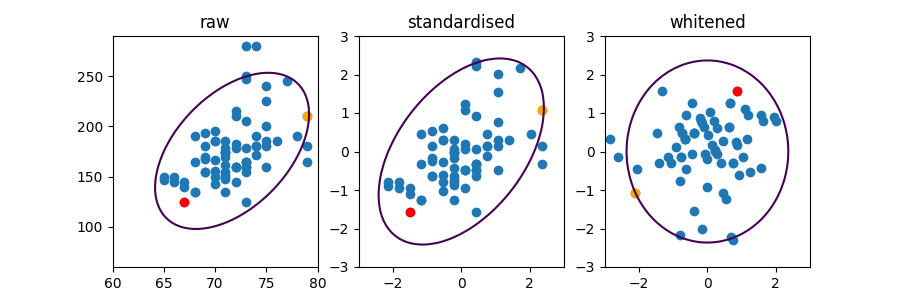
\includegraphics[width=\linewidth]{4-gaussian-models/48-whiten-stdise}
\end{figure}

%\section{Logistic regression}

\end{document}